\chapter{Sprint 1 : Fondations}

\section{Introduction}
Le Sprint~1 livre l'ossature porteuse de \nova{}~: le schéma de
base de données multi-locataire, la couche de sécurité par
Row-Level Security, le flux d'authentification, la plomberie du
webhook WhatsApp et le cerveau IA qui transforme les messages
clients en rendez-vous réservés. L'objectif fixé pour ce sprint
était d'atteindre un état où une seule entreprise peut être créée,
son numéro de téléphone enregistré auprès de Meta, et où un client
réel peut réserver un rendez-vous de bout en bout sans aucune
intervention humaine.

\section{Backlog du Sprint 1}
Le Sprint~1 couvre les \emph{user stories} fondatrices~:
authentification, création de compte, gestion du catalogue de
services, conversation WhatsApp et rappels. Chaque story est
dimensionnée en jours-homme.

\begin{table}[H]
  \centering\small
  \caption{Backlog du Sprint 1 : user stories et effort estimé.}
  \label{tab:bk-s1}
  \renewcommand{\arraystretch}{1.4}
  \begin{tabular}{|p{1.4cm}|>{\raggedright\arraybackslash}p{9.5cm}|>{\centering\arraybackslash}p{2.0cm}|}
    \hline\hline
    \textbf{ID} & \textbf{User story (résumé)} & \textbf{Effort (j)} \\
    \hline
    US01 & Inscription email + lien magique.                          & 1   \\
    \hline
    US02 & Choix du type d'entreprise et valeurs sectorielles.        & 1   \\
    \hline
    US03 & Création et gestion du catalogue de services.              & 1,5 \\
    \hline
    US05 & Configuration du réceptionniste IA.                        & 1   \\
    \hline
    US07 & Création / modification manuelle d'un rendez-vous.         & 1,5 \\
    \hline
    US08 & Historique complet d'un client.                            & 1   \\
    \hline
    US21 & Conversation WhatsApp multilingue.                         & 2   \\
    \hline
    US22 & Réservation multi-tour (nom, service, date, heure).        & 2,5 \\
    \hline
    US23 & Confirmer / annuler via boutons WhatsApp.                  & 1   \\
    \hline
    US24 & Envoi de document attaché au dossier.                      & 1   \\
    \hline
    US31 & Rappels 24~h avec boutons Confirmer/Annuler.               & 1,5 \\
    \hline
    US32 & Rappels 1~h avant le rendez-vous.                          & 1   \\
    \hline
    \multicolumn{2}{r}{\textbf{Total}} & \textbf{16~j} \\
    \hline\hline
  \end{tabular}
\end{table}

\section{Conception du Sprint 1}

\subsection{Diagramme de cas d'utilisation raffiné du Sprint 1}
À partir du diagramme global du chapitre précédent, je retiens
pour ce sprint les cas d'utilisation directement liés aux
fondations côté Admin (\emph{Se connecter}, \emph{Créer un compte},
\emph{Configurer l'entreprise}, \emph{Gérer les clients},
\emph{Gérer les rendez-vous}), côté Patient
(\emph{Discuter via WhatsApp} -- seul point de contact du patient
avec \nova{}), et côté Système (\emph{Envoyer rappels 24~h/1~h}).

\begin{figure}[!htbp]\centering
\definecolor{indS1}{RGB}{99,102,241}
\definecolor{oranS1}{RGB}{251,146,60}
\definecolor{cyanS1}{RGB}{34,211,238}
\begin{tikzpicture}[
  >=Stealth,
  uc/.style={ellipse, draw=indS1!70!black, line width=1.4pt, fill=indS1!12,
    minimum width=3.6cm, minimum height=0.7cm,
    font=\scriptsize, align=center, inner sep=2pt},
  act/.style={font=\scriptsize\bfseries, align=center},
  ext/.style={rectangle, rounded corners=4pt, line width=1.4pt, draw=cyanS1!70!black,
              fill=cyanS1!15, minimum width=1.8cm, minimum height=0.8cm,
              align=center, font=\scriptsize\bfseries},
  sys/.style={rectangle, rounded corners=4pt, line width=1.4pt, draw=oranS1!70!black,
              fill=oranS1!15, minimum width=1.8cm, minimum height=0.8cm,
              align=center, font=\scriptsize\bfseries},
  link/.style={-, draw=gray!70, line width=0.8pt}
]
% Acteurs principaux (gauche)
\node[act] (admin) at (-5.4, 2.0)  {Admin};
\node[act] (pat)   at (-5.4,-2.5)  {Patient};

% Acteurs secondaires (droite)
\node[ext] (wa)     at ( 5.6,-1.5)  {WhatsApp\\(externe)};
\node[sys] (sysExt) at ( 5.6,-3.2)  {Système\\(externe)};

% Cas d'utilisation
\node[uc] (loginA)  at (0, 3.0)  {Se connecter (Admin)};
\node[uc] (createA) at (0, 2.0)  {Créer un compte (Admin)};
\node[uc] (config)  at (0, 1.0)  {Configurer l'entreprise};
\node[uc] (clients) at (0, 0.0)  {Gérer les clients};
\node[uc] (rdv)     at (0,-1.0)  {Gérer les rendez-vous};
\node[uc] (chat)    at (0,-2.5)  {Discuter via WhatsApp};
\node[uc] (rappel)  at (0,-3.5)  {Envoyer rappels 24~h/1~h};

% Liaisons admin
\draw[link] (admin) -- (loginA);
\draw[link] (admin) -- (createA);
\draw[link] (admin) -- (config);
\draw[link] (admin) -- (clients);
\draw[link] (admin) -- (rdv);

% Liaisons patient (uniquement WhatsApp)
\draw[link] (pat) -- (chat);

% Vers acteurs secondaires (droite)
\draw[link] (chat)   -- (wa.west);
\draw[link] (rappel) -- (wa.west);
\draw[link] (rappel) -- (sysExt.west);
\end{tikzpicture}
\caption{Diagramme de cas d'utilisation raffiné du Sprint 1.}
\label{fig:uc-s1}
\end{figure}

\subsection{Descriptions textuelles des cas d'utilisation}

\begin{table}[H]
  \centering\small
  \caption{Description textuelle : Se connecter / Créer un compte (Admin).}
  \label{tab:uc-s1-login-admin}
  \renewcommand{\arraystretch}{1.45}
  \begin{tabular}{|p{3.0cm}|>{\raggedright\arraybackslash}p{10.8cm}|}
    \hline\hline
    \textbf{Nom du cas} & Se connecter / Créer un compte (Admin) \\
    \hline
    \textbf{Acteur principal} & Administrateur \\
    \hline
    \textbf{Acteur secondaire} & Supabase Auth (lien magique e-mail) \\
    \hline
    \textbf{Précondition} & L'admin dispose d'une adresse e-mail valide. \\
    \hline
    \textbf{Scénario nominal} &
      (1) l'admin saisit son e-mail sur la page d'accueil~;
      (2) Supabase Auth envoie un lien magique à usage unique~;
      (3) l'admin clique sur le lien~;
      (4) un jeton JWT est délivré et stocké côté navigateur~;
      (5) à la première connexion, l'admin choisit le type d'entreprise
          et la ligne \texttt{businesses} est créée avec
      \texttt{owner\_user\_id = auth.uid()}. \\
      \hline
    \textbf{Scénario alternatif} & Lien expiré : l'admin demande un
      nouveau lien depuis la même page. \\
      \hline
    \textbf{Postcondition} & Session active~; toutes les requêtes
      PostgREST sont filtrées par RLS sur le \texttt{business\_id}
      de l'admin. \\
    \hline\hline
  \end{tabular}
\end{table}

\begin{table}[H]
  \centering\small
  \caption{Description textuelle : Gérer les clients (Admin).}
  \label{tab:uc-s1-clients}
  \renewcommand{\arraystretch}{1.45}
  \begin{tabular}{|p{3.0cm}|>{\raggedright\arraybackslash}p{10.8cm}|}
    \hline\hline
    \textbf{Nom du cas} & Gérer les clients \\
    \hline
    \textbf{Acteur principal} & Administrateur authentifié \\
    \hline
    \textbf{Précondition} & Session admin active. \\
    \hline
    \textbf{Scénario nominal} &
      (1) l'admin ouvre l'onglet \emph{Clients}~;
      (2) il consulte la liste complète des clients de son entreprise
          (recherche par nom ou téléphone)~;
      (3) il peut consulter la fiche détaillée d'un client
          (historique RDV, messages, documents)~;
      (4) il peut ajouter un client manuellement, modifier ses
          informations ou désactiver son compte~;
      (5) toutes les opérations sont écrites via PostgREST sous RLS
          sur le \texttt{business\_id} de l'admin. \\
          \hline
    \textbf{Postcondition} & La base \texttt{clients} reflète les
      modifications~; le tableau de bord est rafraîchi en temps réel
      via Supabase Realtime. \\
    \hline\hline
  \end{tabular}
\end{table}

\begin{table}[H]
  \centering\small
  \caption{Description textuelle : Configurer l'entreprise.}
  \label{tab:uc-s1-config}
  \renewcommand{\arraystretch}{1.45}
  \begin{tabular}{|p{3.0cm}|>{\raggedright\arraybackslash}p{10.8cm}|}
    \hline\hline
    \textbf{Nom du cas} & Configurer l'entreprise \\
    \hline
    \textbf{Acteur principal} & Administrateur authentifié \\
    \hline
    \textbf{Précondition} & Compte entreprise créé, session active. \\
    \hline
    \textbf{Scénario nominal} &
      (1) l'admin ouvre l'onglet \emph{Services}~;
      (2) il ajoute chaque service (nom, durée, prix, catégorie)~;
      (3) il définit les heures de travail (sept jours, intervalles ouvrables)~;
      (4) il configure les options IA (langue par défaut, FAQ). \\
      \hline
    \textbf{Postcondition} & Le catalogue, les heures et la
      configuration IA sont persistés en base sous RLS du
      \texttt{business\_id} de l'admin. \\
    \hline\hline
  \end{tabular}
\end{table}

\begin{table}[H]
  \centering\small
  \caption{Description textuelle : Discuter via WhatsApp (réservation multi-tour).}
  \label{tab:uc-s1-chat}
  \renewcommand{\arraystretch}{1.45}
  \begin{tabular}{|p{3.0cm}|>{\raggedright\arraybackslash}p{10.8cm}|}
    \hline\hline
    \textbf{Nom du cas} & Discuter via WhatsApp \\
    \hline
    \textbf{Acteur principal} & Patient \\
    \hline
    \textbf{Acteur secondaire} & WhatsApp (canal externe), Claude Haiku (IA) \\
    \hline
    \textbf{Précondition} & Numéro Meta enregistré pour l'entreprise~;
      webhook configuré. \\
      \hline
    \textbf{Scénario nominal} &
      (1) le patient envoie un message libre sur le numéro Meta~;
      (2) Meta livre le message au webhook \texttt{whatsapp-webhook}~;
      (3) le message est persisté dans \texttt{messages}~;
      (4) \texttt{classify-message} appelle Claude Haiku pour extraire
          \texttt{\{intent, language, entities\}}~;
      (5) si \texttt{intent = book\_appointment}, la machine d'états
          collecte les champs manquants~;
      (6) une ligne \texttt{appointments} est insérée~;
      (7) \nova{} répond par WhatsApp avec un message de confirmation. \\
      \hline
    \textbf{Scénario alternatif} & Intention non reconnue~: \nova{}
      renvoie une FAQ ou demande une reformulation. \\
      \hline
    \textbf{Postcondition} & Rendez-vous créé en base et confirmé
      au patient via WhatsApp. \\
    \hline\hline
  \end{tabular}
\end{table}

\begin{table}[H]
  \centering\small
  \caption{Description textuelle : Envoyer rappels 24~h / 1~h.}
  \label{tab:uc-s1-rappel}
  \renewcommand{\arraystretch}{1.45}
  \begin{tabular}{|p{3.0cm}|>{\raggedright\arraybackslash}p{10.8cm}|}
    \hline\hline
    \textbf{Nom du cas} & Envoyer rappels 24~h / 1~h \\
    \hline
    \textbf{Acteur principal} & Système (agent automatisé) \\
    \hline
    \textbf{Acteur secondaire} & WhatsApp \\
    \hline
    \textbf{Déclencheur} & \texttt{pg\_cron} toutes les 10~minutes. \\
    \hline
    \textbf{Scénario nominal} &
      (1) la fonction \texttt{send-reminders} sélectionne les
          rendez-vous dans la fenêtre cible~;
      (2) elle envoie un message WhatsApp avec deux boutons
          (Confirmer, Annuler)~;
      (3) la réponse du patient est interceptée par
          \texttt{whatsapp-webhook} qui met à jour le statut~;
      (4) les drapeaux \texttt{reminder\_sent\_*} sont mis à vrai
          pour éviter les doublons. \\
          \hline
    \textbf{Postcondition} & Le statut du rendez-vous reflète la
      réponse du patient~; aucun doublon de rappel n'est envoyé. \\
    \hline\hline
  \end{tabular}
\end{table}

\section{Design du Sprint 1}

\subsection{Diagrammes de séquence du Sprint 1}
À chaque cas d'utilisation du Sprint~1 correspond un diagramme de
séquence présenté ci-dessous. Tous les diagrammes sont générés à
partir de fichiers PlantUML situés dans
\texttt{figures/sources/seq-s1-*.puml}.

\paragraph{Se connecter / Créer un compte (Admin).}
La figure~\ref{fig:seq-s1-login-admin} décrit le flux
d'authentification par lien magique e-mail de l'administrateur via
Supabase Auth.

\begin{figure}[!htbp]\centering
\IfFileExists{figures/seq-s1-login-admin.png}{%
  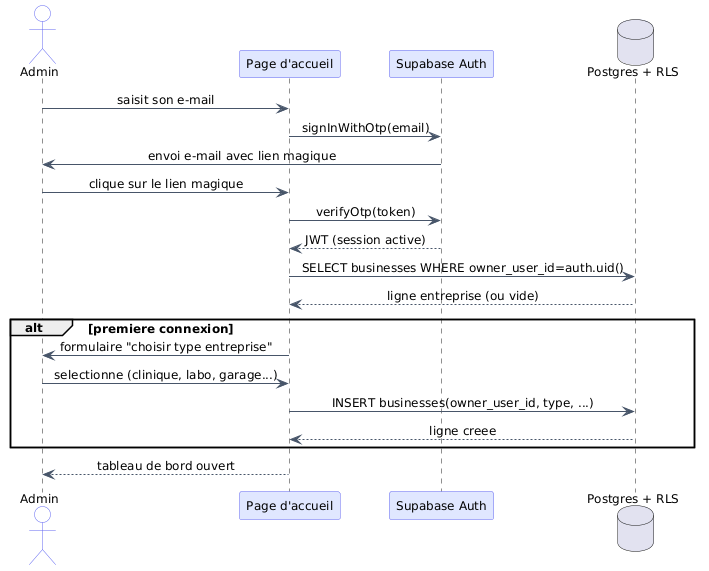
\includegraphics[width=.95\textwidth,height=.55\textheight,keepaspectratio]{figures/seq-s1-login-admin.png}%
}{\fbox{\parbox[c][4cm][c]{.85\textwidth}{\centering\itshape\small[seq-s1-login-admin.puml -- a generer via plantuml.com]}}}
\caption{Diagramme de séquence : Se connecter / Créer un compte (Admin).}
\label{fig:seq-s1-login-admin}
\end{figure}

\paragraph{Discuter via WhatsApp (réservation).}
La figure~\ref{fig:seq-s1-chat} détaille la réservation
multi-tour~: réception du message, classification d'intention par
Claude Haiku, machine d'états de prise de RDV, confirmation.

\begin{figure}[!htbp]\centering
\IfFileExists{figures/seq-s1-chat-whatsapp.png}{%
  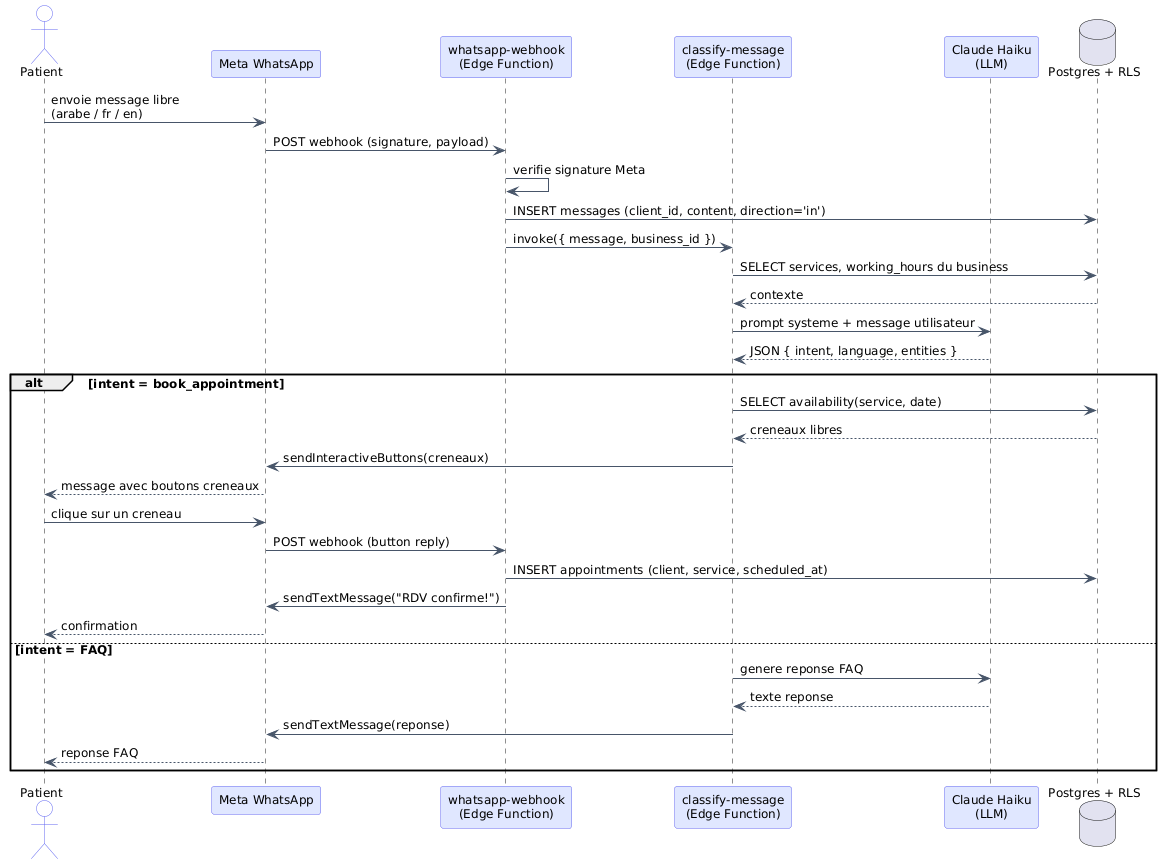
\includegraphics[width=.95\textwidth,height=.6\textheight,keepaspectratio]{figures/seq-s1-chat-whatsapp.png}%
}{\fbox{\parbox[c][4cm][c]{.85\textwidth}{\centering\itshape\small[seq-s1-chat-whatsapp.puml -- a generer via plantuml.com]}}}
\caption{Diagramme de séquence : Discuter via WhatsApp et réserver un rendez-vous.}
\label{fig:seq-s1-chat}
\end{figure}

\paragraph{Envoyer rappels 24~h / 1~h.}
La figure~\ref{fig:seq-s1-rappels} montre le cron périodique, la
sélection des RDV éligibles, l'envoi des boutons interactifs et la
mise à jour du statut.

\begin{figure}[!htbp]\centering
\IfFileExists{figures/seq-s1-rappels.png}{%
  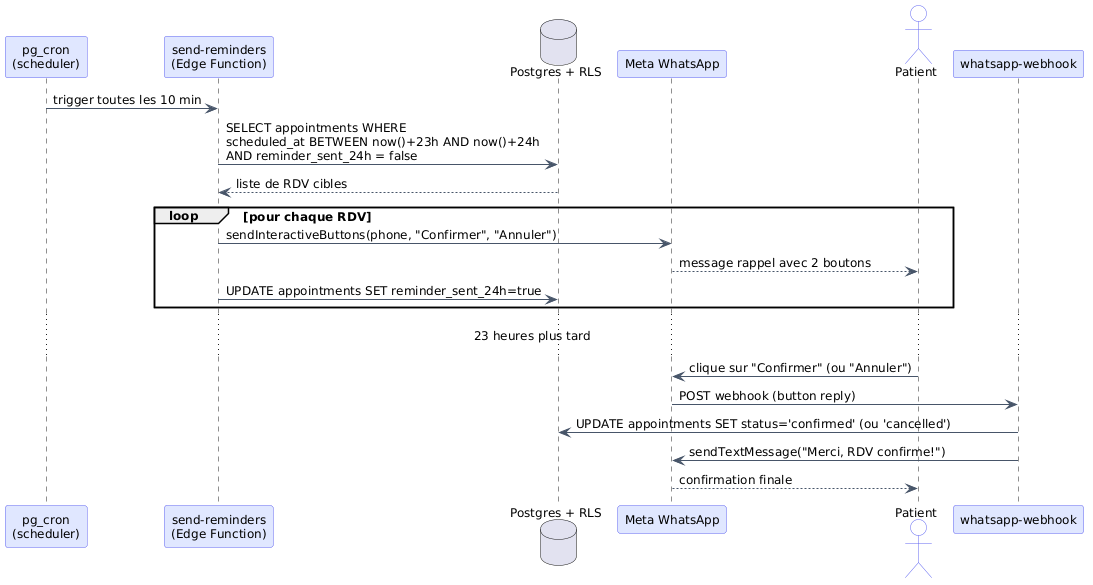
\includegraphics[width=1.10\textwidth,height=.6\textheight,keepaspectratio]{figures/seq-s1-rappels.png}%
}{\fbox{\parbox[c][4cm][c]{.85\textwidth}{\centering\itshape\small[seq-s1-rappels.puml -- a generer via plantuml.com]}}}
\caption{Diagramme de séquence : Envoyer rappels 24~h / 1~h.}
\label{fig:seq-s1-rappels}
\end{figure}

\section{Implémentation du Sprint 1}

\subsection{Schéma de la base de données}
Le schéma central, défini dans \texttt{schema.sql}, comporte sept
tables plus leurs index et contraintes de clé étrangère~:
\texttt{businesses}, \texttt{users} (équipe), \texttt{clients},
\texttt{services}, \texttt{appointments}, \texttt{messages} et
\texttt{notifications}. Plutôt que de modifier directement
\texttt{schema.sql} à chaque ajout, j'ai adopté une discipline de
migrations \emph{idempotentes}~: chaque évolution structurelle est
un nouveau fichier numéroté dans \texttt{migrations/}, et chaque
migration est écrite de manière à être rejouable plusieurs fois
sans erreur.

\subsection{Row-Level Security multi-locataire}
Chaque table métier porte une politique RLS qui filtre les lignes
par \texttt{business\_id} appartenant à l'admin connecté
(\texttt{auth.uid()}). La politique type est~:
\texttt{business\_id IN (SELECT id FROM businesses WHERE
owner\_user\_id = auth.uid())}. Aucune logique de filtrage
multi-locataire n'est nécessaire côté frontend~: la base elle-même
applique la barrière.

\subsection{Authentification et création de compte (Admin)}
La connexion utilise le lien magique fourni par Supabase Auth. Le
flux d'onboarding consiste à saisir un e-mail, recevoir un lien à
usage unique, puis choisir un type d'entreprise dans la liste
supportée. La figure~\ref{fig:auth-signin} montre l'écran
d'inscription par e-mail, et la figure~\ref{fig:setup-business}
montre le formulaire de création d'entreprise qui suit (nom, type,
numéro WhatsApp, choix du plan d'abonnement).

\begin{figure}[!htbp]\centering
\includegraphics[width=.92\textwidth,keepaspectratio]{figures/auth-signin.jpg}
\caption{Écran d'inscription : email + lien magique.}\label{fig:auth-signin}
\end{figure}

\begin{figure}[!htbp]\centering
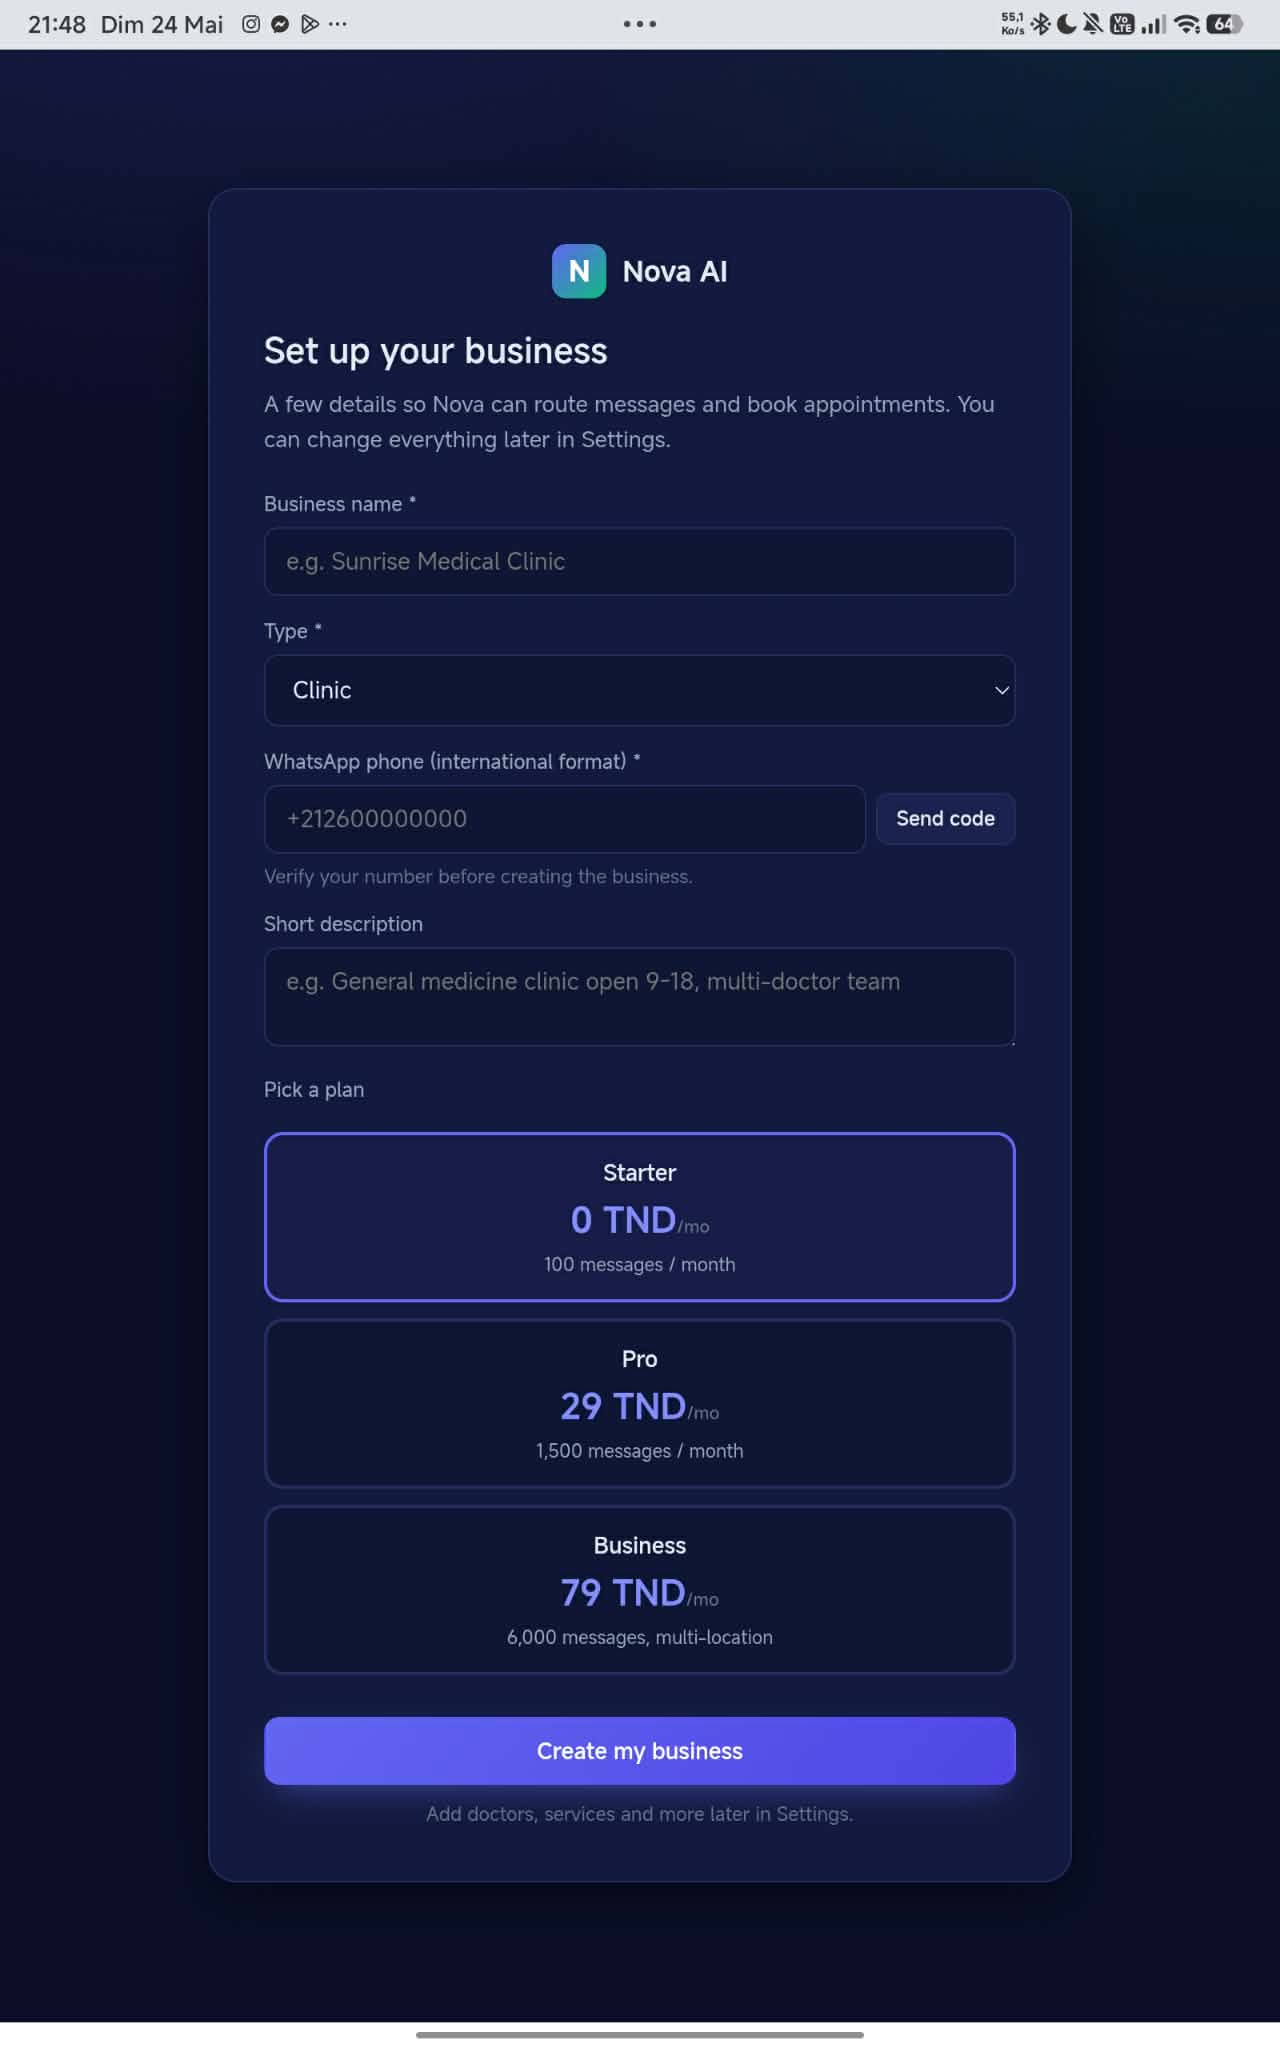
\includegraphics[width=.55\textwidth,keepaspectratio]{figures/setup-business.jpg}
\caption{Formulaire de création d'entreprise : nom, type, WhatsApp, plan d'abonnement.}\label{fig:setup-business}
\end{figure}

\subsection{Webhook WhatsApp et classifieur d'intention}
La fonction Edge \texttt{whatsapp-webhook} vérifie la signature
Meta, persiste le message entrant et délègue la décision à
\texttt{classify-message}. Cette dernière construit un prompt
système qui inclut le catalogue de services, les heures
d'ouverture et le sigle de langue cible, puis appelle Claude Haiku.
La sortie est un JSON strict \texttt{\{intent, language,
entities\}} consommé par la machine d'états.

\subsection{Discuter via WhatsApp -- parcours utilisateur}
Les figures suivantes illustrent le parcours réel du patient sur
WhatsApp, capturé sur des conversations test avec le numéro Meta
de \nova{}.

La figure~\ref{fig:wa-arabic} montre une réservation conduite
principalement en arabe dialectal puis en français, avec le rappel
templaté envoyé la veille du rendez-vous.

\begin{figure}[!htbp]\centering
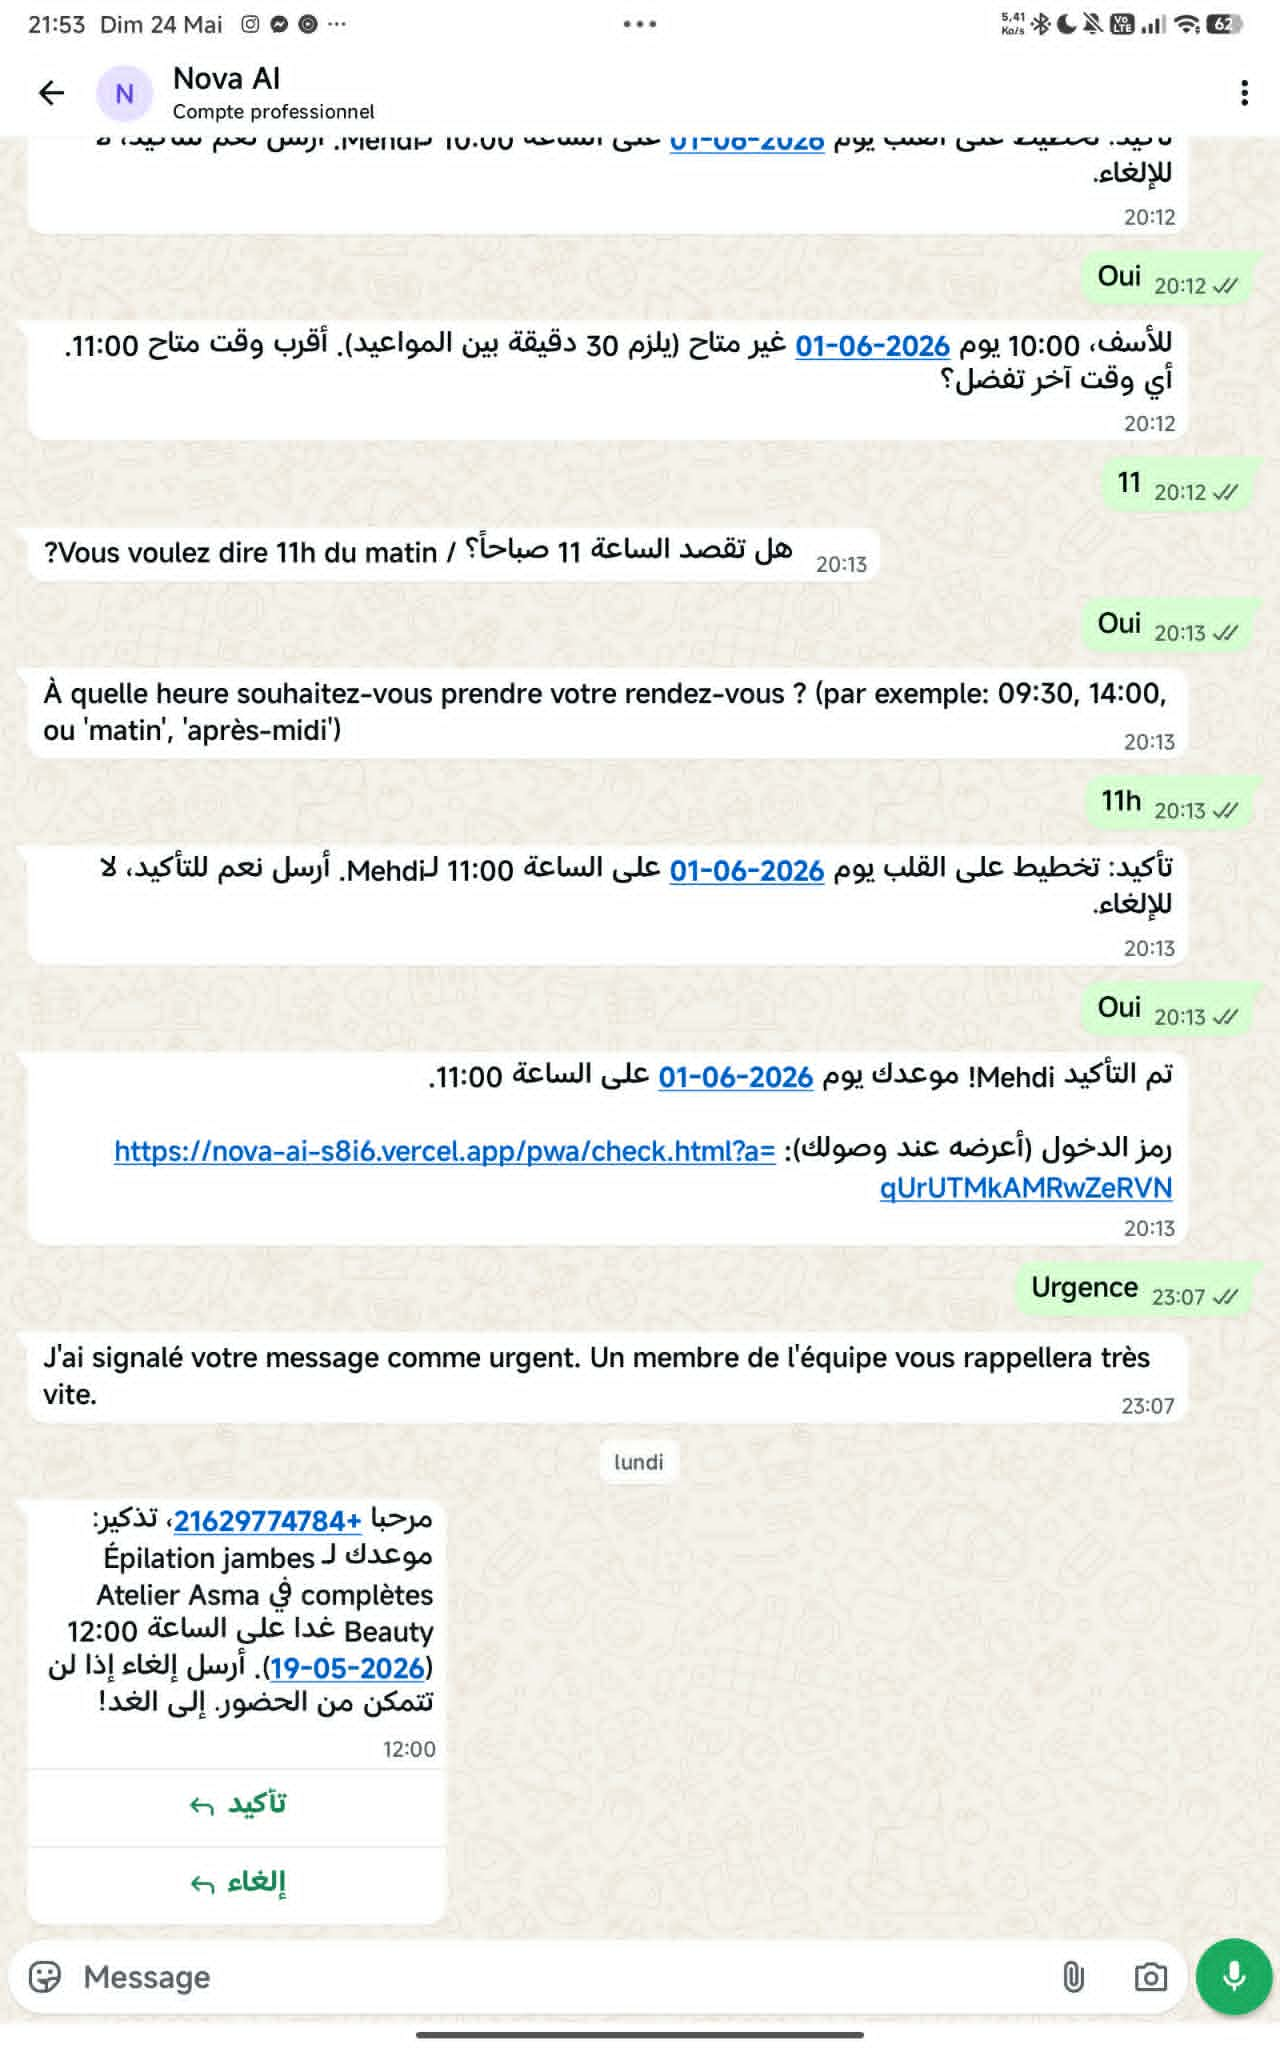
\includegraphics[width=.55\textwidth,keepaspectratio]{figures/whatsapp-booking-arabic.jpg}
\caption{Conversation WhatsApp : réservation multilingue et rappel 24~h.}\label{fig:wa-arabic}
\end{figure}

La figure~\ref{fig:wa-voice} montre la prise de rendez-vous à
partir de messages vocaux WhatsApp~: \nova{} transcrit chaque
audio via Whisper avant de l'envoyer au classifieur Claude Haiku.

\begin{figure}[!htbp]\centering
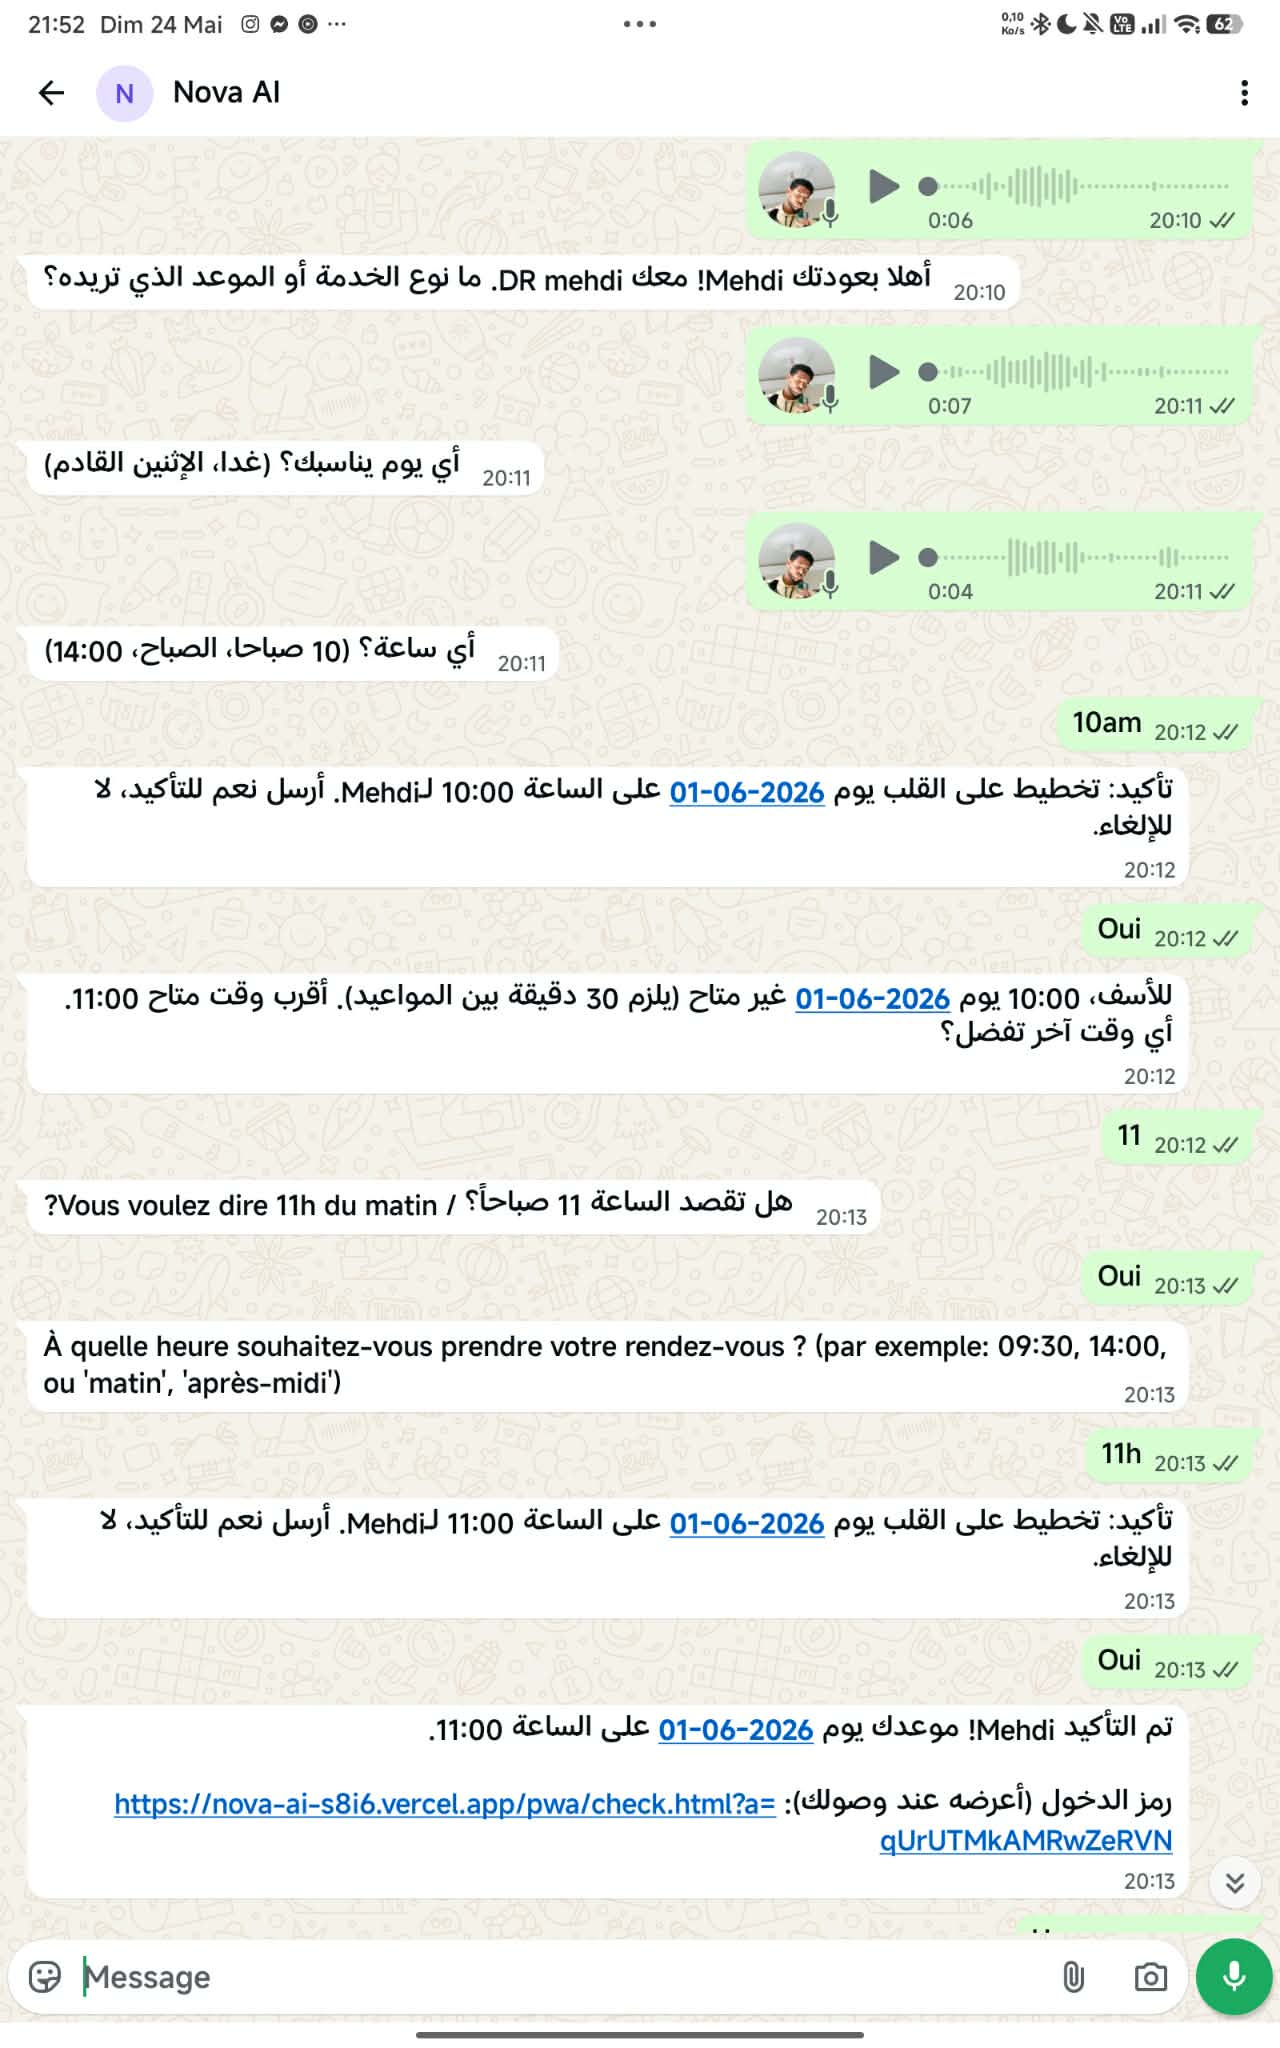
\includegraphics[width=.55\textwidth,keepaspectratio]{figures/whatsapp-booking-voice.jpg}
\caption{Conversation WhatsApp : prise de rendez-vous à partir de messages vocaux.}\label{fig:wa-voice}
\end{figure}

La figure~\ref{fig:wa-lab} montre le parcours d'un laboratoire
d'analyses~: confirmation avec liste des analyses et prix,
gestion d'un créneau déjà pris, lien de check-in et publication
automatique du résultat.

\begin{figure}[!htbp]\centering
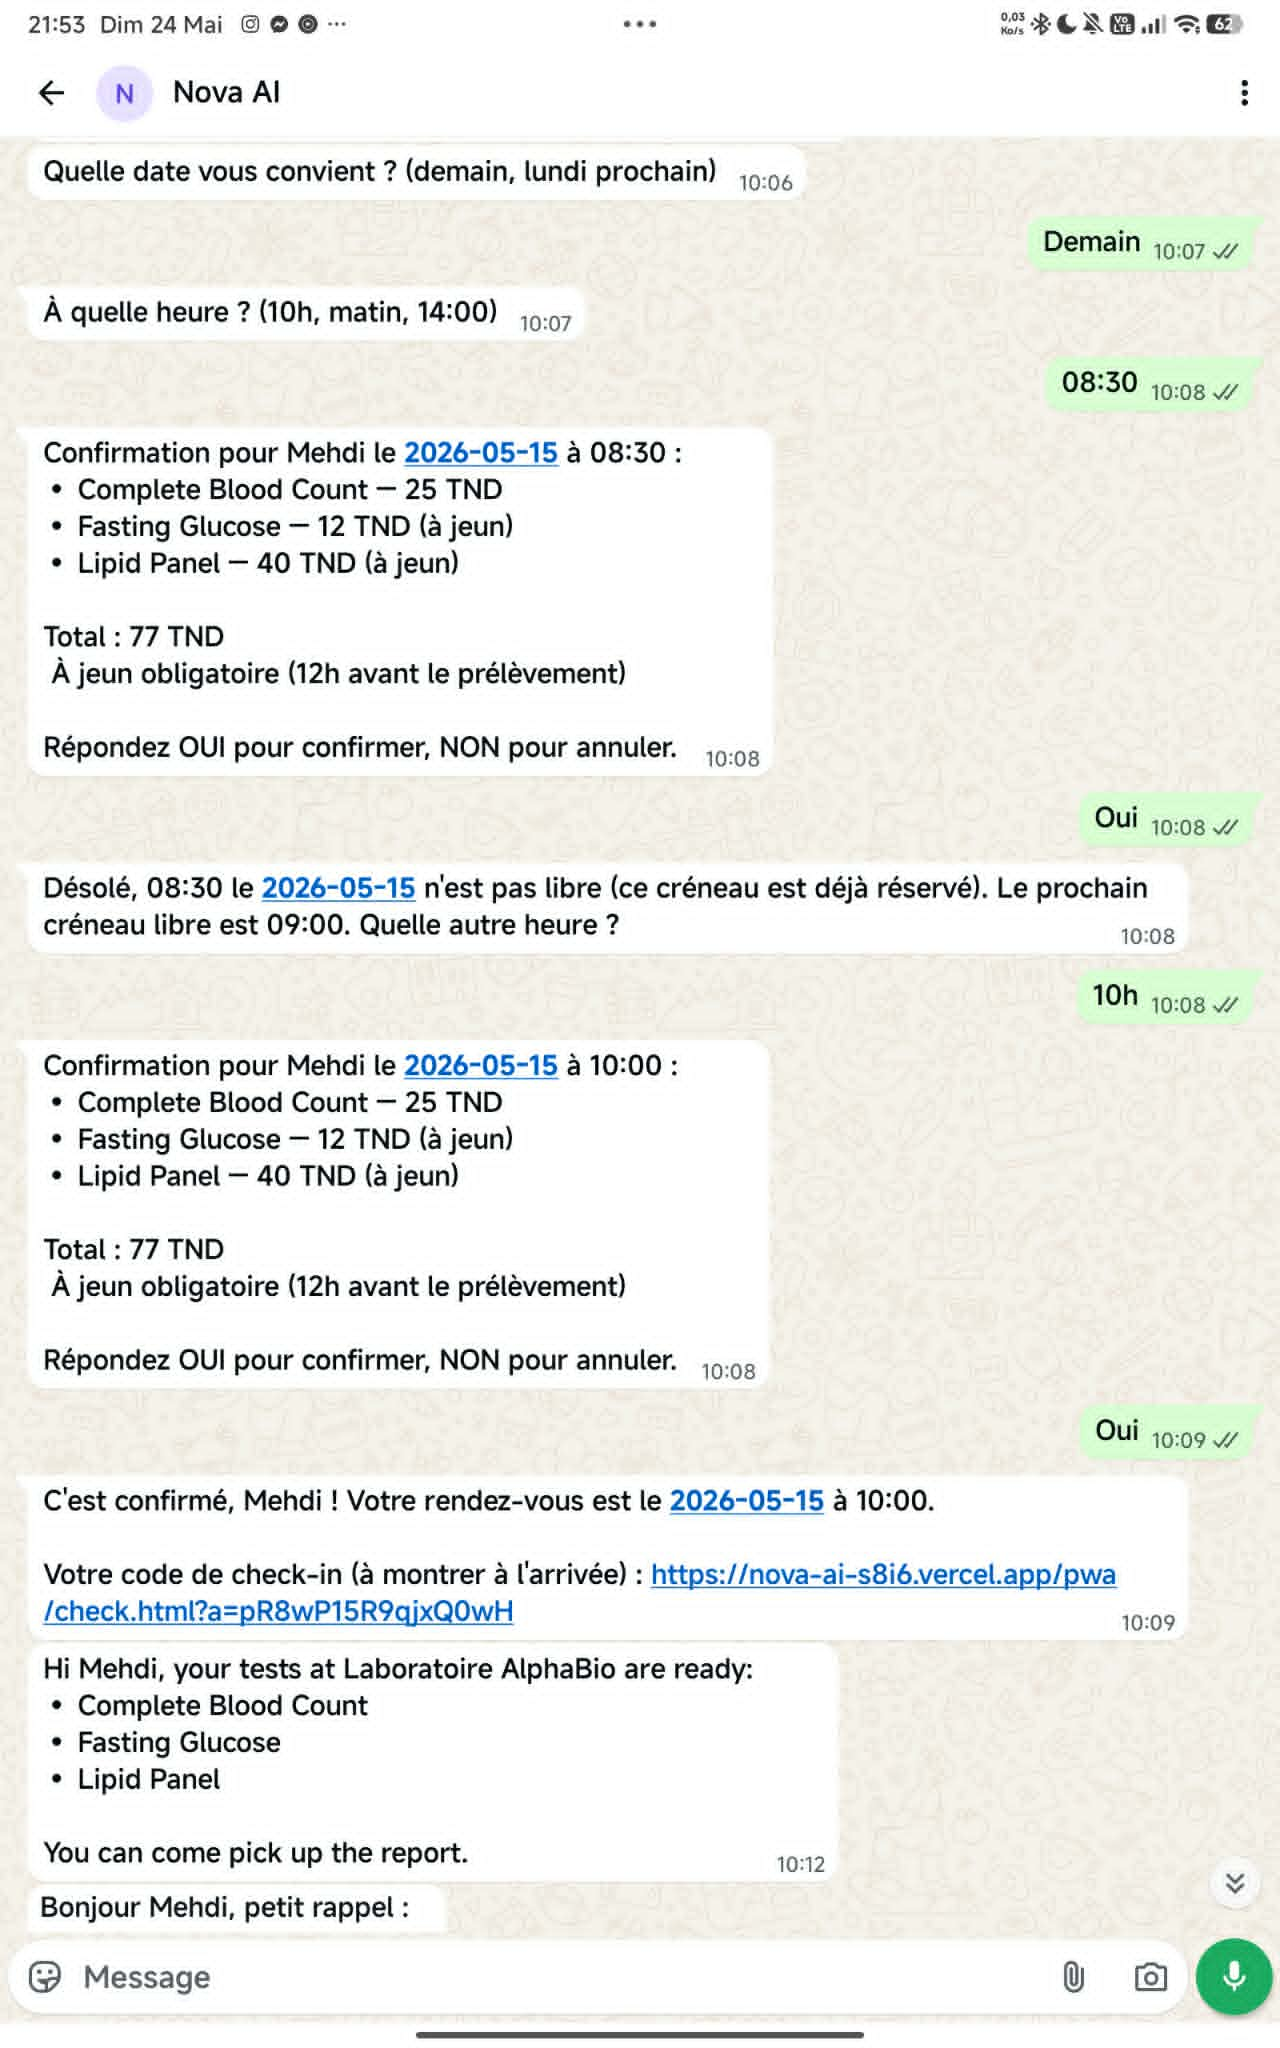
\includegraphics[width=.55\textwidth,keepaspectratio]{figures/whatsapp-booking-lab.jpg}
\caption{Conversation WhatsApp : parcours laboratoire complet (réservation, confirmation, check-in, résultats).}\label{fig:wa-lab}
\end{figure}

\section{Tests unitaires et revue du Sprint 1}
Pour chaque \emph{user story} du Sprint~1, j'ai écrit un test
minimal exécuté avant la clôture~:
\begin{itemize}
  \item \textbf{Authentification.} Envoi d'un lien magique, clic,
        vérification que \texttt{auth.uid()} est non nul.
  \item \textbf{RLS.} Tentative de lecture d'une table d'un autre
        \texttt{business\_id} via un JWT valide~; le résultat doit
        être vide.
  \item \textbf{Classifieur.} Jeu de 30 messages annotés (10 par
        langue)~; l'intention doit être correcte sur 90\,\% des
        cas.
  \item \textbf{Webhook.} Rejouer manuellement un \emph{payload}
        Meta et vérifier que la ligne \texttt{messages} est créée
        puis traitée idempotemment (la rejouer une seconde fois
        ne doit pas créer de doublon).
  \item \textbf{Rappels.} Insérer un rendez-vous à T+24~h,
        déclencher \texttt{send-reminders} manuellement, vérifier
        qu'un WhatsApp est envoyé et que
        \texttt{reminder\_sent\_24h} passe à vrai.
\end{itemize}

La revue de sprint avec mon encadrante a validé que le parcours
bout-en-bout fonctionne~: un client réel envoie un message, \nova{}
extrait l'intention, propose un créneau et inscrit le rendez-vous,
sans aucune intervention humaine.

\section{Conclusion}
Le Sprint~1 a livré l'ossature de \nova{}~: un schéma
multi-locataire isolé par RLS, une authentification administrateur
sans mot de passe, un webhook WhatsApp idempotent et un
classifieur d'intention multilingue. Cette fondation rend possible
le Sprint~2, qui ajoute les surfaces opérationnelles (tableau de
bord, gestion des rendez-vous et des clients) et la PWA patient.
